% Glava dokumenta
\documentclass{beamer}
\usepackage[slovene]{babel}
\usepackage[utf8]{inputenc}
\usepackage{lmodern}
\usepackage[T1]{fontenc}
\usepackage{amsthm}
\usepackage{amsmath}
\usepackage{listings}
\usepackage{amssymb}
\usepackage{graphicx}
\usepackage{url}
\usepackage{multirow}
\usetheme{Warsaw}
\setbeamercovered{transparent}
%\usecolortheme{crane}
\title[Verjetnost prekomernega prileganja]{VERJETNOST PREKOMERNEGA PRILEGNJA}
\author[Tina Janša]{Tina Janša}


\begin{document}


\begin{frame}
\titlepage
\end{frame}


\begin{frame}
\frametitle{Uvod}

%\begin{block}{Naloga}
%Za dani nabor trgovalnih strategij izračunaj verjetnost prekomernega prileganja z novo metodo kombinatoričnega simetričnega navzkrižnega preverjanja.
%\end{block}
%\vspace{0.5cm}
\begin{itemize}
\item Pridobitev podatkov \pause
\item Implementacija trgovalnih strategij 
\item Implementacija metode kombinatoričnega simetričnega navzkrižnega preverjanja
\end{itemize}

\end{frame}


%\begin{frame}
%\frametitle{Podatki}
%S\&P 500 - borzni indeks, ki temelji na tržni kapitalizaciji 500 velikih podjetji, katerih navadne delnice kotirajo na Newyorški borzi ali NASDAQ
%\end{frame}

\begin{frame}
\frametitle{Trgovalne strategije}
\begin{itemize}
\item Random \pause
\item Buy \& Hold \pause
\item SMA
\item RSI
\item Bollinger
\end{itemize}
\end{frame}


\begin{frame}
\frametitle{SMA - Preprosto drseče povprečje}
\begin{itemize}
\item Nakupni signal: zadnja cena > SMA
\item Prodajni signal: zadnja cena < SMA
\end{itemize}

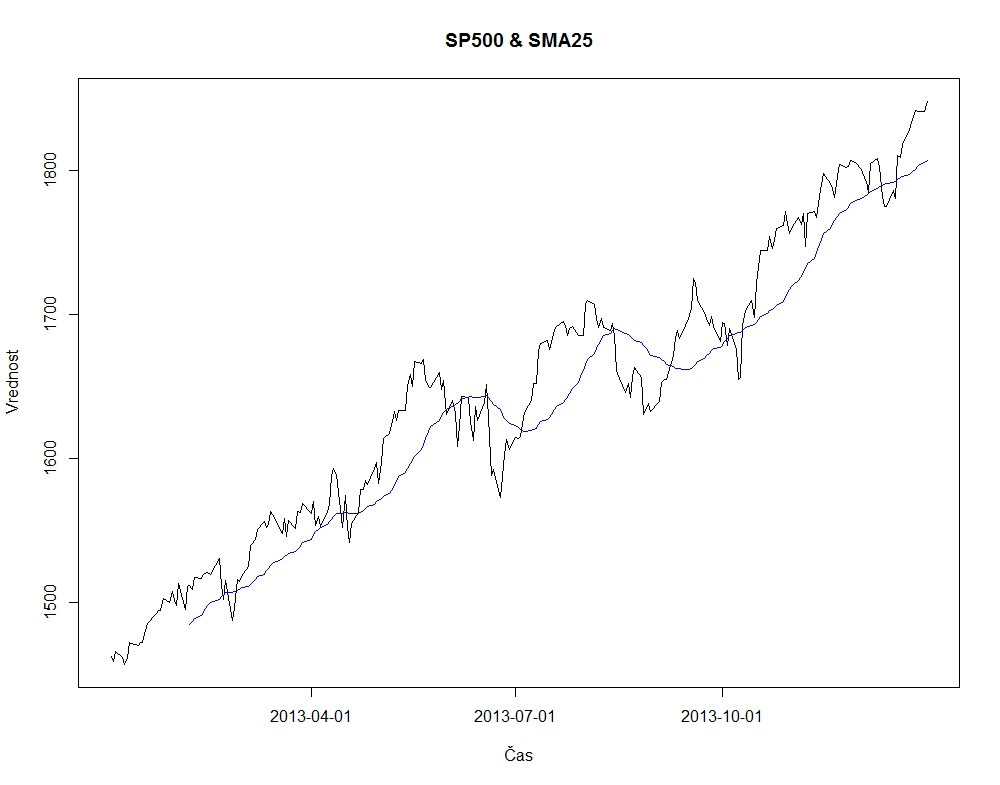
\includegraphics[width=10cm]{SMA25.png}

\end{frame}


\begin{frame}
\frametitle{RSI - Indeks relativne moči}
\begin{columns}
\begin{column}{5cm}
\begin{itemize}
\item Nakupni signal: RSI < 30
\item Prodajni signal: RSI > 70
\end{itemize}

$$RSI = 100 - \frac{100}{1-RS}$$

\end{column}

\begin{column}{6.3cm}
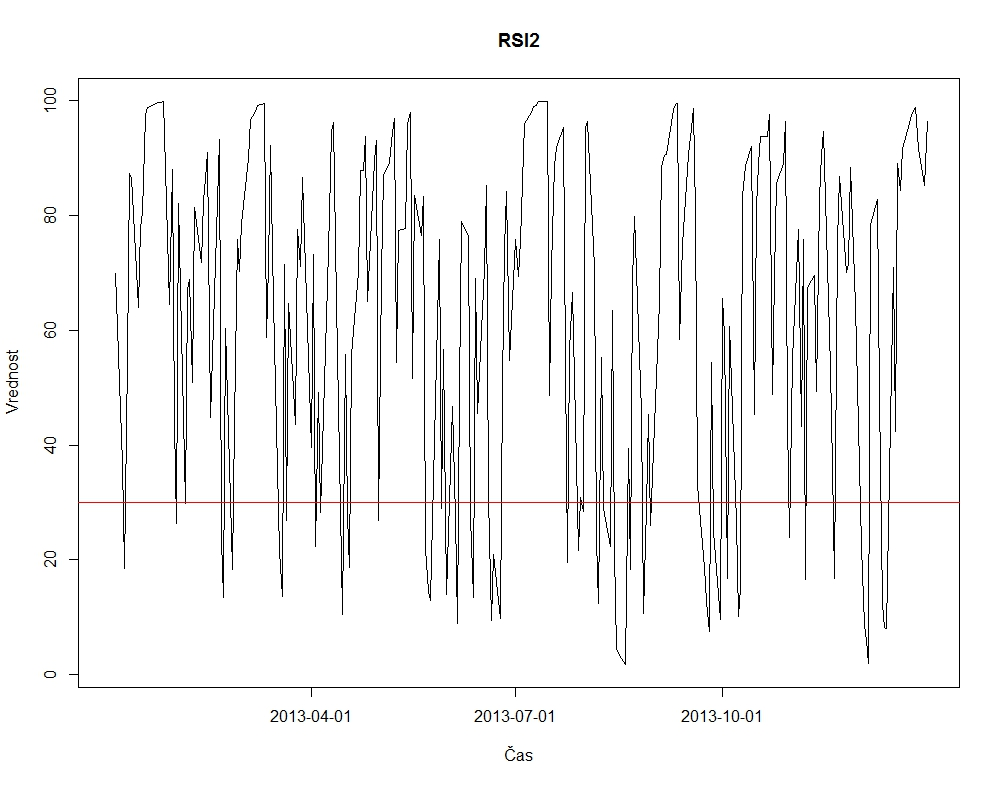
\includegraphics[width=6.3cm]{RSI2.png}
\end{column}
\end{columns}
\vspace{0.5cm}
$$RS = \frac{\textrm{povprečna vrednost pozitivnih period}}{\textrm{povprečna vrednost negativnih period}}$$
\end{frame}


\begin{frame}
\frametitle{Bollingerjevi pasovi}
\begin{itemize}
\item Nakupni signal: zadnja cena < spodnji pas
\item Prodajni signal: zadnja cena > zgornji pas
\end{itemize}
\begin{itemize}
\item zgornji pas = SMA + faktor $\times$ standardni odklon
\item srednji pas = SMA
\item spodnji pas = SMA - faktor $\times$ standardni odklon
\end{itemize}
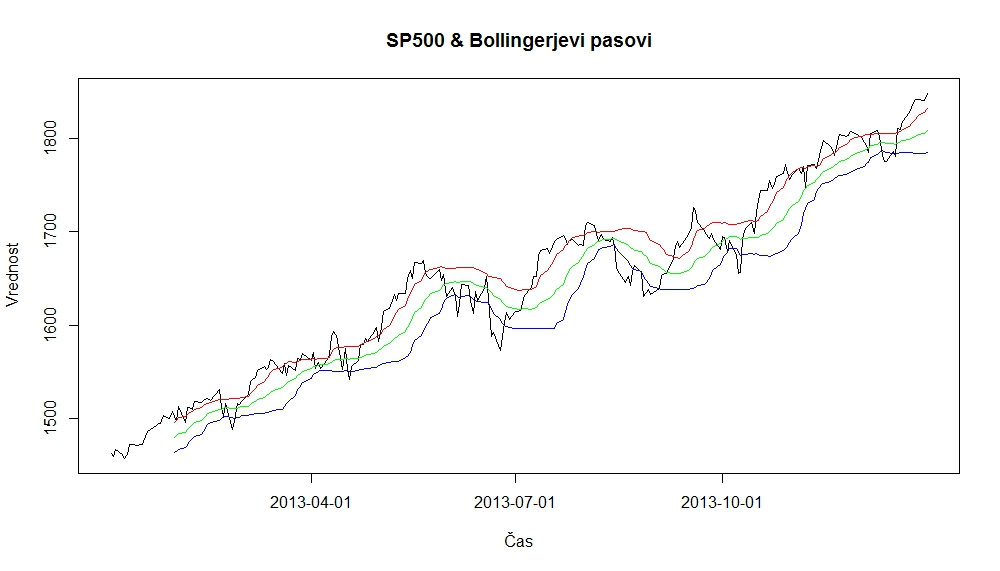
\includegraphics[width=10cm]{Bollinger.png}

\end{frame}


\begin{frame}
\frametitle{Trgovalne strategije}
\includegraphics[width=11cm]{kapital_5let.png}
\end{frame}

\begin{frame}
\frametitle{Metoda kombinatoričnega simetričnega navzkrižnega preverjanja}
\begin{itemize}
\item Prekomerno prileganje: najboljša strategija na učni množici je zelo slaba na testni množici
\item Verjetnost prekomernega prileganja
\item Sharpovo razmerje: mera uspešnosti strategije
\end{itemize}
\end{frame}


\begin{frame}[allowframebreaks,t]
\frametitle{CSCV - Metoda kombinatoričnega simetričnega prečnega preverjanja}
\begin{enumerate}
\item	Konstruiramo matriko $M$ iz časovne vrste uspešnosti $N$ strategij. $M$ je matrika velikosti $T\times N$. 
\item	$M$ razdelimo po vrsticah na $S$ disjunktnih podmatrik enakih velikosti. Vsaka od teh podmatrik $M_s$, $s=1,\dots,S$, je velikosti $\frac{T}{S} \times N$.
\item	Tvorimo kombinacije $\frac{S}{2}$ podmatrik $M_s$, kar nam da ${S \choose \frac{S}{2}}$ kombinacij $C_s$. 
\item	Za vsako kombinacijo $c \in C_s$ naredimo naslednje:
\begin{itemize}
\item	Konstruiramo učno množico $J$ tako da združimo $\frac{S}{2}$ podmatrik $M_s$, ki so v kombinaciji $c$. $J$ je matrika velikosti $\frac{T}{2} \times N$.
\item	Konstruiramo testno množico $\overline{J}$ iz podmatrik, ki niso v $J$.
\item	Konstruiramo vektor $R$, kjer $n$-ti element pove uspešnost $n$-tega stolpca matrike $J$.
\item	Določimo element $n^*$ tako, da je $R_n \leq R_n^*$, $\forall n = 1,\dots,N$.
\item	Konstruiramo vektor $\overline{R}$, kjer $n$-ti element pove uspešnost $n$-tega stolpca matrike $\overline{J}$.
\item	Določimo relativni rank $\overline{R_n^*}$ v $\overline{R}$. Označimo ga z $\overline{\omega_c}$, kjer je $\overline{\omega_c} \in (0,1)$. 
\item	Definiramo logit $\lambda_c = log\frac{\overline{\omega_c}}{1-\overline{\omega_c}}$. $\lambda_c = 0$, ko je $\overline{R_n^*} = Me[\overline{R}]$.
\end{itemize}
\item	Izračunamo porazdelitev rankov testne množice z zbiranjem vseh $\lambda_c$, za $c \in C_s$. $f(\lambda)$ je relativna frekvenca pri kateri se $\lambda$ zgodi na vseh $C_s$, z $\int_{-\infty}^{\infty} f(\lambda)d\lambda = 1$.
\item Verjetnost prekomernega prileganja lahko ocenimo z $\Phi = \int_{-\infty}^{0}f(\lambda)d\lambda$.
\begin{itemize}
\item $\Phi \approx 0$: ni velikega prekomernega prileganja, ker je izbor optimalne strategije na učni množici pripomogel k večji uspešnosti na testni množici.
\item $\Phi = \frac{1}{2}$: zgodovinsko preverjanje se prekomerno prilega do te mere, da postopek izbora optimalne strategije na učni množici ne doda vrednosti.
\item $\Phi >> \frac{1}{2}$: prekomerno prileganje je tako veliko, da izbor optimalne strategije na učni množici povzroči slabšo pričakovano uspešnost na testni množici, kot bi bila, če bi naključno izbrali eno izmed strategij.
\end{itemize}
\end{enumerate}
\end{frame}


%\begin{frame}
%\frametitle{Rezultati}
%{\footnotesize
%\begin{tabular}{|p{1.15cm}|p{0.8cm}|p{1.4cm}|p{1.4cm}|p{1.2cm}|p{1.2cm}|p{1.2cm}|}
%\cline{3-7}
%\multicolumn{2}{c|}{}&\multicolumn{5}{|c|}{\textbf{STRATEGIJE}}\\
%\cline{3-7}
%\multicolumn{2}{c|}{} & SMA150 & SMA150 & RSI2 & RSI2 & \multirow{5}{1cm}{vse strategije} \\
%\multicolumn{2}{c|}{} & RSI14 & RSI14 & Bollinger & Bollinger & \\
%\multicolumn{2}{c|}{} & Buy\&Hold &  Buy\&Hold  & Random & Random & \\
%\multicolumn{2}{c|}{} & & SMA50 & & SMA25 & \\
%\multicolumn{2}{c|}{} & & Random &   & RSI14 &  \\
%\hline
%\multirow{2}{*}{\textbf{CSCV}} & 5 let & 0.7953 & 0.8038 & 0.0004 & 0.0026 & 0.1060 \\
% & 13 let & 0.7416 & 0.7025 & 0.0017 & 0.0039 & 0.0333 \\
%\hline
%\multirow{2}{*}{\textbf{Hold-out}} & 5 let & 3 & 5 & 3 & 5 & vse \\
% & 13 let & 3 & 5 & 3 & 5 & vse \\
% \hline
%\end{tabular}
%}
%\end{frame}

\begin{frame}
\frametitle{Rezultati}
\begin{tabular}{|c|c|c|c|c|}
\hline
SMA150 & SMA150 & RSI2 & RSI2 & \multirow{5}{*}{vse strategije} \\
RSI14 & RSI14 & Bollinger & Bollinger & \\
Buy\&Hold &  Buy\&Hold  & Random & Random & \\
& SMA50 & & SMA25 & \\
 & Random &   & RSI14 &  \\
\hline
 0.7953 & 0.8038 & 0.0004 & 0.0026 & 0.1060 \\
 \hline
\end{tabular}
\end{frame}



\begin{frame}
\includegraphics[width=11cm]{velik_overfit_3strategije_5let.png}
\end{frame}

\begin{frame}
\includegraphics[width=11cm]{velik_overfit_5strategij_5let.png}
\end{frame}

%\begin{frame}
%\includegraphics[width=11cm]{velik_overfit_3strategije_13let.png}
%\end{frame}

%\begin{frame}
%\includegraphics[width=11cm]{velik_overfit_5strategij_13let.png}
%\end{frame}

\begin{frame}
\includegraphics[width=11cm]{majhen_overfit_3strategije_5let.png}
\end{frame}

\begin{frame}
\includegraphics[width=11cm]{majhen_overfit_5strategij_5let.png}
\end{frame}

%\begin{frame}
%\includegraphics[width=11cm]{majhen_overfit_3strategije_13let.png}
%\end{frame}

%\begin{frame}
%\includegraphics[width=11cm]{majhen_overfit_5strategij_13let.png}
%\end{frame}

\begin{frame}
\includegraphics[width=11cm]{kapital_5let.png}
\end{frame}

%\begin{frame}
%\includegraphics[width=11cm]{kapital_13let.png}
%\end{frame}




\end{document} 
